\documentclass{beamer}
\usecolortheme{wolverine}

% math stuff
\usepackage{amsmath}
\usepackage{amsthm}
\usepackage{amssymb}
\usepackage{xcolor}

\usepackage{float}
\usepackage{subcaption}

% to insert images
\usepackage{graphicx}

% to correctly insert stressed characters
\usepackage[T1]{fontenc}
\usepackage[utf8]{inputenc}

\usepackage{multirow}

% Bibliography
% \usepackage[style=alphabetic]{biblatex}
% \usepackage[nottoc]{tocbibind}
% \usepackage{bibentry}
% \setcounter{biburllcpenalty}{9000}
% \usepackage{nameref}
% \addbibresource{slides.bib}

% to put links in table of contents
\usepackage{hyperref}
\hypersetup{colorlinks=false, %set true if you want colored links
	linktoc=all,     %set to all if you
}

\usepackage{mathtools}

% Add symbols
% \usepackage{textcomp}

% Add command for Real and Z sets
% \usepackage{dsfont}
% \newcommand{\Rset}{$\mathds{R}$}
% \newcommand{\Zset}{$\mathds{Z}$}

% Code highlighting
% \usepackage{minted}
% \usemintedstyle{perldoc}
% \setminted{
%     frame=single,
%     breaklines,
% }

% tikz figures
% \usepackage{tikzit}
% \input{style.tikzstyles}

% number rounding
\usepackage{siunitx}
\sisetup{round-mode=places,round-precision=5}

\definecolor{myyellow}{RGB}{225, 225, 0}

\title{Thesis notes}
\date{18th May}

% any code between @(...)@ is escaped back to LaTeX
% \lstset{escapeinside={@(}{)@}}

% algorithms
\usepackage[ruled,vlined]{algorithm2e}
% \newtheorem{theorem}{Theorem}

\begin{document}

\frame{\titlepage}

\begin{frame}[c]
	\frametitle{The Echo Chamber Problem - notation}

	\begin{itemize}
		\item $G = (V, E ^{+}, E ^{-}) $ interaction graph
		\item $ \mathcal{C} $ set of contents
		\item $C \in \mathcal{C} $ content, $\mathcal{T} _{C} $ set of threads
		      associated with $C$. A thread $T \in \mathcal{T} _{C} $ is a
		      subgraph of $G$
		      % So $G = \bigcup _{C
		      % \in \mathcal{C} } \bigcup _{T \in \mathcal{T} _C} T $ union of all
		      % threads of all contents
		\item $U \subseteq V$ subset of users, $T[U]$ subgraph of $T$ induced
		      by $U$. $|T(U)|$ is the number of edges of this subgraph
	\end{itemize}
\end{frame}

\begin{frame}[c]
	\frametitle{The Echo Chamber Problem - notation}
	\begin{itemize}
		\item $\eta(C)$ fraction of negative edges associated with $C$
		      (analogous definition for a thread $T$). Content (or thread)
		      controversial if $\eta \in (\alpha, 1]$
		\item $\hat{\mathcal{C} } \subseteq \mathcal{C} $ set of \textit{controversial}
		      contents

		\item $\mathcal{S} _C (U)$ set of \textit{non controversial} threads
		      induced by $U$, for \textit{controversial} contents, i.e.

			      {\small
				      \begin{equation}
					      \mathcal{S} _{C} (U) = \{ T[U] \; s.t. \; T[U] \; non \;
					      controversial, T \in \mathcal{T} _{C}, C
					      \in \hat{\mathcal{C}}, U \subseteq V\}
				      \end{equation}
			      }
	\end{itemize}

\end{frame}

\begin{frame}[c]
	\frametitle{The Echo Chamber Problem}
	\textbf{Goal}: given an interaction graph $G$, find $U \subseteq V$ maximing

	\begin{equation}
		\xi (U) = \sum^{}_{C \in \hat{\mathcal{C}} } \sum^{}_{T[U] \in S_C (U)}
		(| T^{+} [U] | - | T^{-} [U] |)
	\end{equation}

	where $| T^{-} [U] |$ and $| T^{+} [U] |$ denotes the number of negative
	and positive edges induced in the subgraph, respectively.

	\bigskip

	The set of users maximing the expression is denoted as $\hat{U}$ and the
	corresponding score is $\xi(G)$
\end{frame}

\begin{frame}[c]
	\frametitle{Computing exactly the score}
	\begin{equation}
		maximize \; \sum_{ T_{k} \in \mathcal{T}_{C}, \; C \in
			\mathcal{\hat{C}} } \big( \sum^{}_{ij \in E^{+} (T_{k})} x_{ij}
			^{k} - \sum_{ij \in E^{-} (T_{k})} x_{ij} ^{k} \big)
	\end{equation}
	\begin{equation}
		x _{ij}^{k}  \leq y_i, \; x _{ij} ^{k} \leq y_j, \;x _{ij}^{k}  \leq z_k \quad\quad \forall ij \in E(T_{k}), T_{k} \in
		\mathcal{T}_{C}, C \in \mathcal{\hat{C}}
	\end{equation}
	\begin{equation}
		x _{ij} ^{k} \geq - 2 + y_i + y_j + z_k \quad\quad \forall ij \in E(T_k), T_k \in \mathcal{T} _{C}, C \in \hat{\mathcal{C} }
	\end{equation}
	\begin{equation}
		\sum^{}_{ij \in E^{-} (T_k)} x_{ij}^{k}  - \alpha \sum^{}_{ij \in E(T_k)}
		x_{ij} ^{k}  \leq 0 \quad\quad \forall T_{k} \in \mathcal{T} _{C}, C \in
		\hat{\mathcal{C}}
	\end{equation}
	\begin{equation}
		y _{i} \in  \{0, 1\} \quad\quad \forall i \in V
	\end{equation}
	\begin{equation}
		0 \leq x _{ij} ^{k}  \leq 1 \quad\quad \forall ij \in E(T_{k}), T_{k} \in
		\mathcal{T}_{C}, C \in \mathcal{\hat{C}}
	\end{equation}
	\begin{equation}
		0 \leq z _{k} \leq 1 \quad\quad \forall T_{k} \in \mathcal{T} _{C}, C \in
		\hat{\mathcal{C}}
	\end{equation}

	For $\alpha \leq 0.5$. Only the objective function needed to be corrected.
\end{frame}

\begin{frame}[c]
	\frametitle{Computing exactly the score}
	For $\alpha > 0.5$ additional constraints and variables are needed.

	\begin{equation}
		\sum^{}_{ij \in E^{-} (T_k)} a_{ij}^{k}  - \alpha \sum^{}_{ij \in E(T_k)}
		a_{ij} ^{k} \geq - N_{k} z_{k}  \quad\quad \forall T_{k} \in \mathcal{T} _{C}, C \in
		\hat{\mathcal{C}}
	\end{equation}
	\begin{equation}
		a_{ij}^{k} \geq -1 + y_i + y_j \quad\quad \forall ij \in E(T_{k}), T_{k} \in
		\mathcal{T}_{C}, C \in \mathcal{\hat{C}}
	\end{equation}
	\begin{equation}
		a_{ij}^{k} \leq y_i, \; a_{ij}^{k} \leq y_j \quad\quad \forall ij \in E(T_{k}), T_{k} \in
		\mathcal{T}_{C}, C \in \mathcal{\hat{C}}
	\end{equation}
	\begin{equation}
		0 \leq a_{ij}^{k} \leq 1 \quad\quad \forall ij \in E(T_{k}), T_{k} \in
		\mathcal{T}_{C}, C \in \mathcal{\hat{C}}
	\end{equation}
	\begin{equation}
		0 \leq z _{k} \in  \{0, 1\} \quad\quad \forall T_{k} \in \mathcal{T} _{C}, C \in
		\hat{\mathcal{C}}
	\end{equation}

	Where $a_{ij} ^{k}  $ encodes the information "$e_{ij}^{k}  $ is induced by the
	chosen set of vertices".

	\bigskip

\end{frame}
\begin{frame}[c]
	\frametitle{Computing exactly the score}
	This because for $\alpha > 0.5 $ there may be non controversial threads
	whose total contribution to the score is negative. Without this constraint
	the model would prefer "considering" them as controversial, i.e. setting
	$z_{k} $ to $0$.

	\bigskip

	With the previous new constraint if the vertices induce a subgraph which is
	not controversial then $z_{k} $ is forced to be $1$, and consequently the
	corresponding $x_{ij}^{k}  $.

	\bigskip

	$N_{k} $ can be chosen to be $\alpha \cdot |E^{-} (T_k)| $, which is the
	minimum value achievable by the $LHS$.

\end{frame}

\begin{frame}[c]
	\frametitle{A model for the Echo Chamber Problem}
	Each node has a group assignment and there are probabilities of
	positive and negative edges $\omega _{rs}^{+}  $ and $\omega _{rs}^{+}  $,
	respectively.

	\begin{enumerate}
		\item Generate the \emph{follow} graph $G$ by using a SBM with parameters
		      $\{ \phi _{rs}  \}$.
		\item Each node can be active with probability $\beta_{a}  $
		\item Any active node activates his inactive neighbours in $G$ with
		      probability $\beta_n$
		      % \item Let $a_{i} $ be the number of \emph{active} neighbours of node
		      %     $i$ in $G$ and $m_{i} $ the number of neighbours of node $i$ in
		      %     $G$. Any node inactive from the previous step is activated with
		      %     probability $ \frac{a_i}{m_i} \beta _{n} $
		\item active nodes interact according to the categorical $(\omega _{rs}
			      ^{+}, \omega _{rs} ^{-}, 1 - \omega _{rs} ^{+} - \omega _{rs} ^{-})
		      $ otherwise (at least one of the 2 nodes is inactive) with
		      categorical $(\theta \omega _{rs} ^{+}, \theta \omega _{rs} ^{-}, 1
			      - \theta (\omega _{rs} ^{+} + \omega _{rs} ^{-}))$, $\theta \leq 1$
	\end{enumerate}

\end{frame}

\begin{frame}[c]
	\frametitle{A parametrized model (1)}
	Parameter choice:
	\begin{equation}
		\phi_{rs}  =
		\begin{cases}
			1 \; & \text{if } r = s  \\
			0 \; & \text{otherwise }
		\end{cases}
	\end{equation}
	Users follow other all and only users in the same community.

	\bigskip

	$\beta _{a} = 1$ , $\beta_{n} = 1 $: all users interact on each post.

	\begin{equation}
		\omega_{rs}^{+}   =
		\begin{cases}
			1 - x \; & \text{if } r = s  \\
			x \;     & \text{otherwise }
		\end{cases}
		\omega_{rs}^{-}   =
		\begin{cases}
			x \;     & \text{if } r = s  \\
			1 - x \; & \text{otherwise }
		\end{cases}
	\end{equation}

	where the \emph{noise} $x$ is distributed according to a Truncated Normal distribution with $\mu = 0$,
	standard deviation $\sigma$ and truncated within the $[0, \; 1]$ interval.

\end{frame}

\begin{frame}[c]
	\frametitle{A parametrized model (2)}

	If there is no \emph{noise} the model will produce a graph with communities
	corresponding to positive cliques while each node will be connected to
	all nodes in the other communities with negative edges.

	\bigskip

	As the noise increases interaction between users in the same community and
	in different communities will become less distinguishable.

	\bigskip

	The tests have been carried on very small graphs since the exact model was
	also used, $10$ nodes per community and $3$ threads.

\end{frame}

\begin{frame}[c]
	\frametitle{A parametrized model - results}

	Even in absence of noise the approximation algorithm is not able to cluster all
	nodes correctly, differently from the exact MIP model.

	\begin{figure}
		\begin{center}
			\begin{subfigure}[b]{0.3\textwidth}
				\centering
				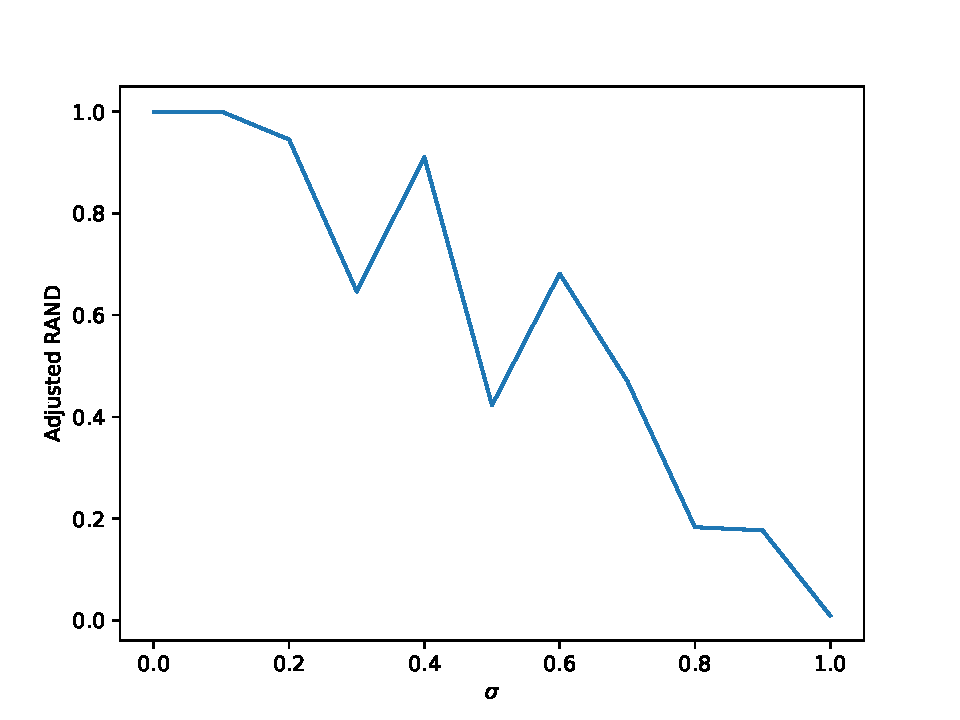
\includegraphics[width=\textwidth]{out/synthetic_exact/model2_sigmas_adj_rand.pdf}
				\caption{Adj RAND, MIP}
				\label{fig:out/synthetic_exact/model2_sigmas_adj_rand.pdf}
			\end{subfigure}
			\begin{subfigure}[b]{0.3\textwidth}
				\centering
				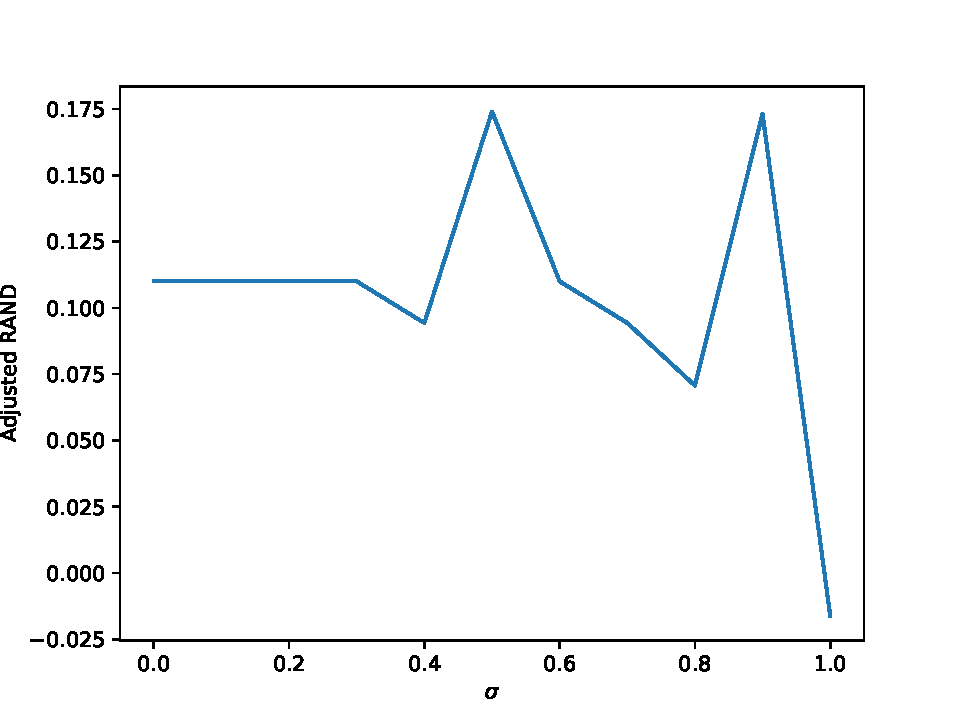
\includegraphics[width=\textwidth]{out/synthetic_appr/model2_sigmas_adj_rand.pdf}
				\caption{Adj RAND, approx.}
				\label{fig:adj-rand-appr1}
			\end{subfigure}
		\end{center}
		\begin{center}
			\begin{subfigure}[b]{0.3\textwidth}
				\centering
				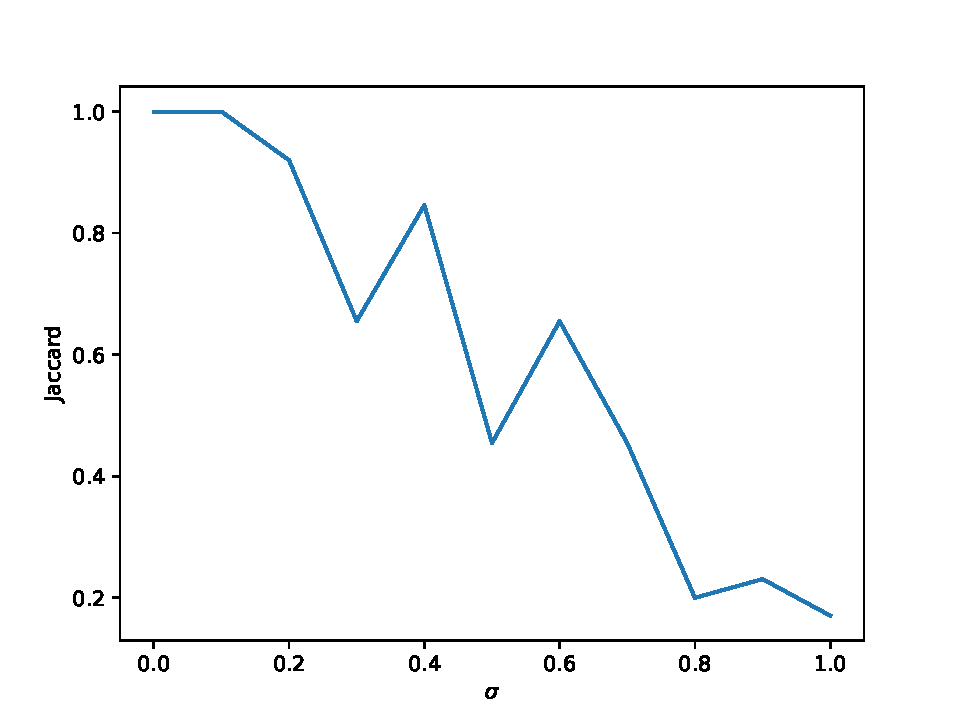
\includegraphics[width=\textwidth]{out/synthetic_exact/model2_sigmas_jaccard.pdf}
				\caption{Jaccard, MIP}
				\label{fig:out/synthetic_exact/model2_sigmas_jaccard.pdf}
			\end{subfigure}
			\begin{subfigure}[b]{0.3\textwidth}
				\centering
				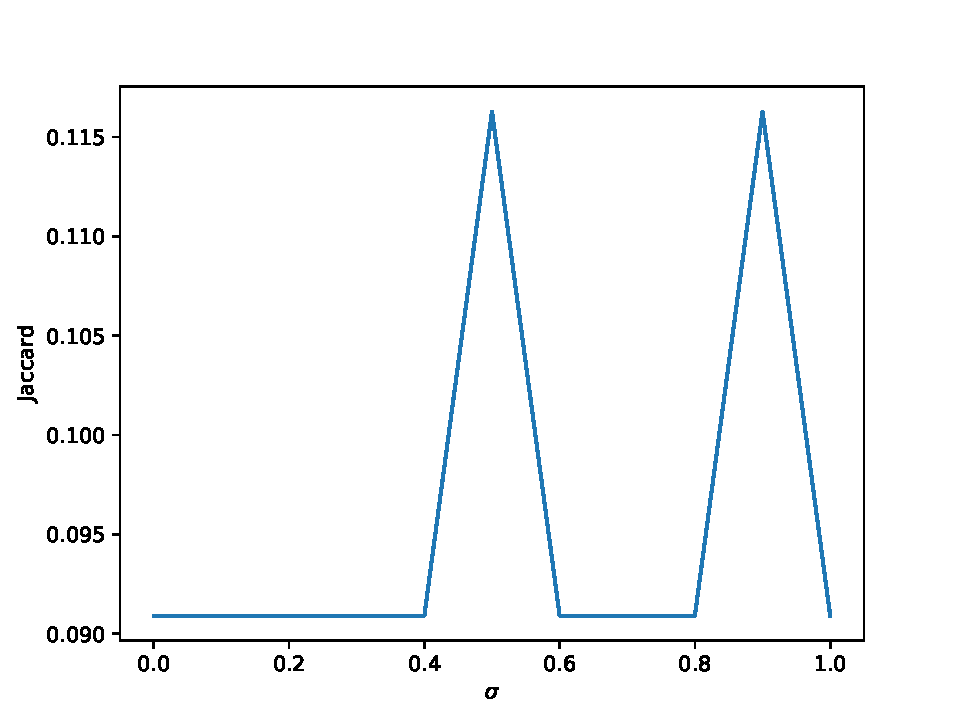
\includegraphics[width=\textwidth]{out/synthetic_appr/model2_sigmas_jaccard.pdf}
				\caption{Jaccard, approx.}
				\label{fig:jacc-appr1}
			\end{subfigure}
		\end{center}
	\end{figure}

\end{frame}

\begin{frame}[c]
	\frametitle{A parametrized model - results}

	MIP is also more robust to noise than the other variants of the problem.

	\begin{figure}
		\begin{center}
			\begin{subfigure}[t]{0.3\textwidth}
				\centering
				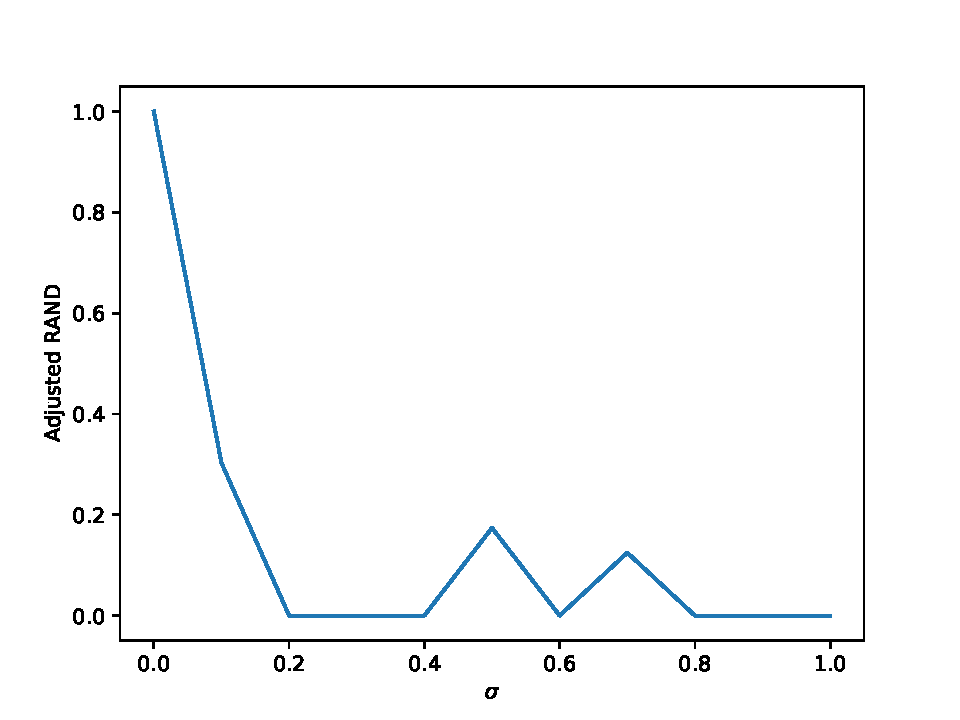
\includegraphics[width=\textwidth]{out/synthetic_densest_nc/model2_sigmas_adj_rand.pdf}
				\caption{Adj RAND, Densest subgraph on Threads}
				\label{fig:out/synthetic_densest_nc/model2_sigmas_adj_rand.pdf}
			\end{subfigure}
			\begin{subfigure}[t]{0.3\textwidth}
				\centering
				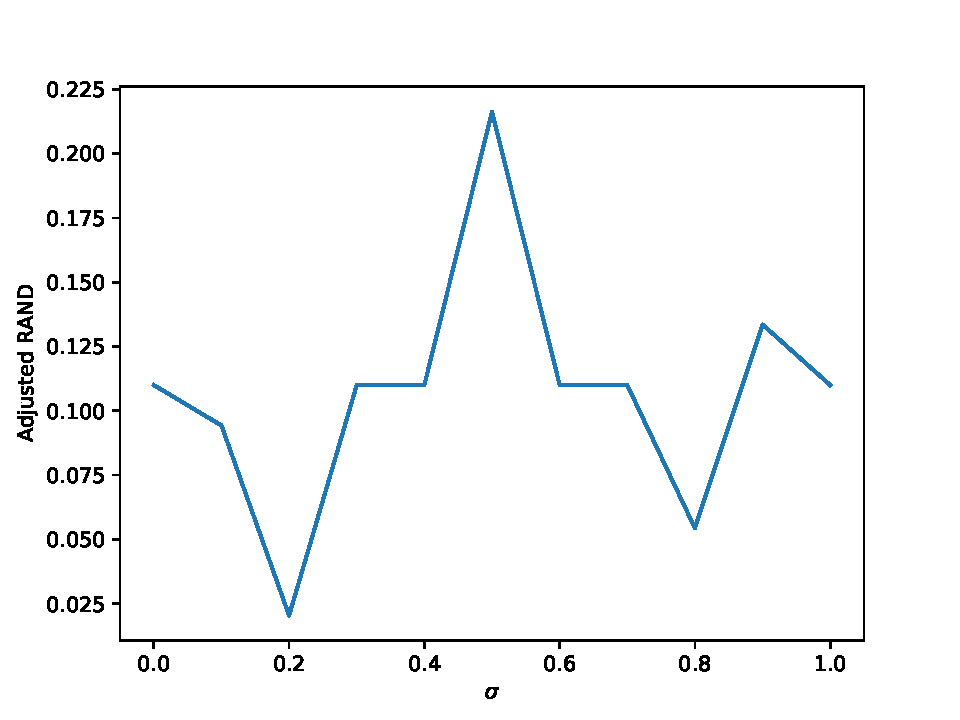
\includegraphics[width=\textwidth]{out/synthetic_o2_bff/model2_sigmas_adj_rand.pdf}
				\caption{Adj RAND, O$^{2}$-BFF}
				\label{fig:adj-rand-o2_bff1}
			\end{subfigure}
		\end{center}
		\begin{center}
			\begin{subfigure}[t]{0.3\textwidth}
				\centering
				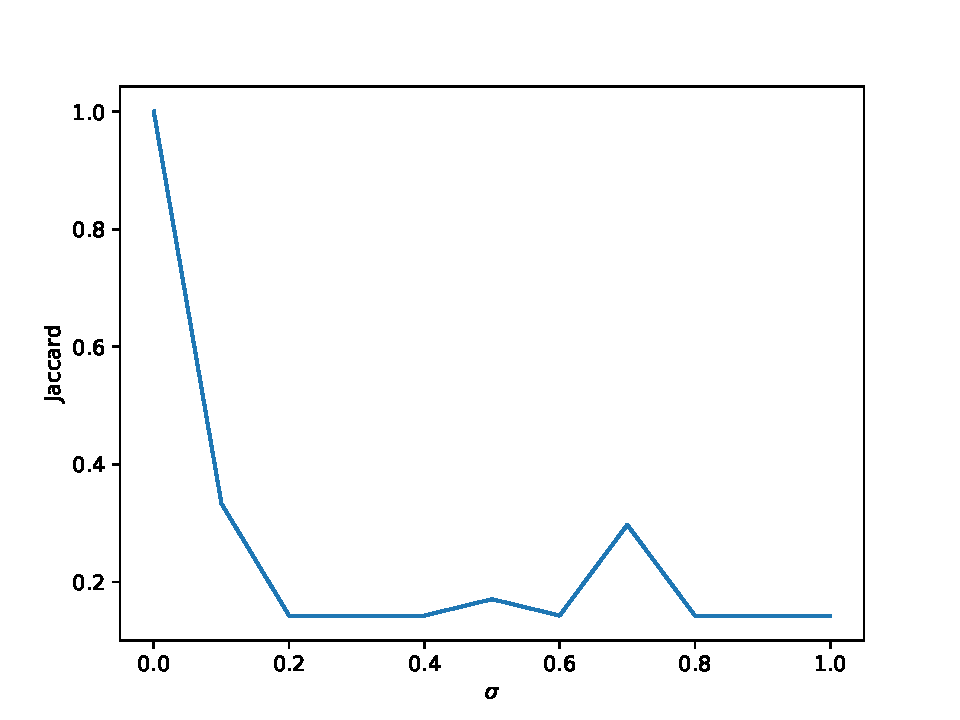
\includegraphics[width=\textwidth]{out/synthetic_densest_nc/model2_sigmas_jaccard.pdf}
				\caption{Jaccard, Densest subgraph on Threads}
				\label{fig:out/synthetic_densest_nc/model2_sigmas_jaccard.pdf}
			\end{subfigure}
			\begin{subfigure}[t]{0.3\textwidth}
				\centering
				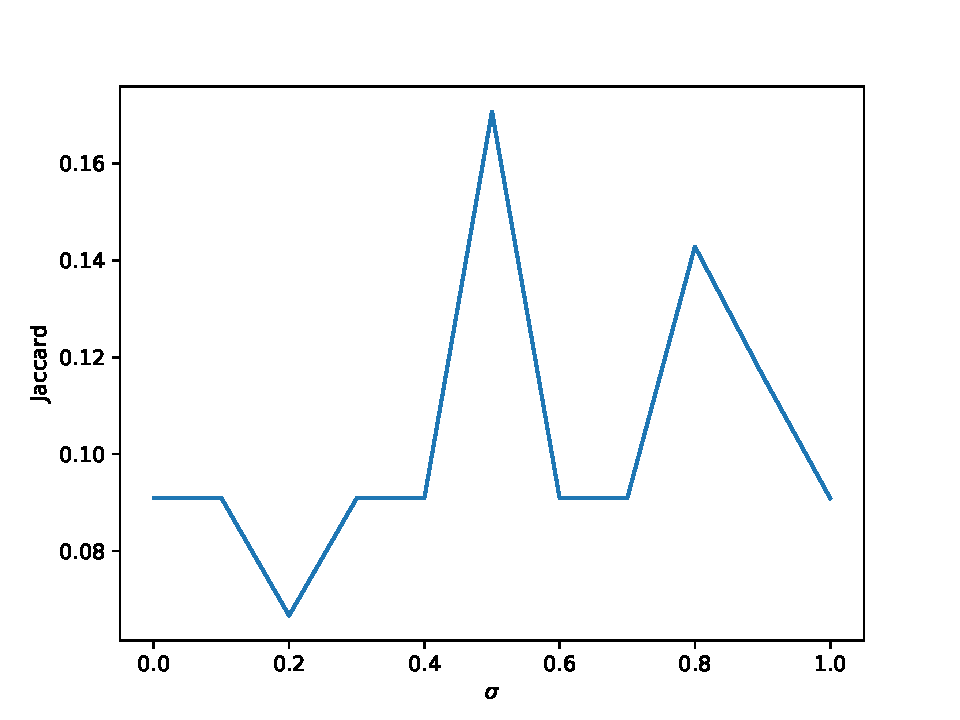
\includegraphics[width=\textwidth]{out/synthetic_o2_bff/model2_sigmas_jaccard.pdf}
				\caption{Jaccard, O$^{2}$-BFF}
				\label{fig:jacc-o2_bff1}
			\end{subfigure}
		\end{center}
	\end{figure}

\end{frame}

\begin{frame}[c]
	\frametitle{Solving exactly the D-ECP}

	{\footnotesize
		\begin{equation}
			maximize \; \sum_{ T_{k} \in \mathcal{T}_{C}, \; C \in
				\mathcal{\hat{C}} } \big( \sum^{}_{ij \in E^{+} (T_{k})} x_{ij}
				^{k} - \sum_{ij \in E^{-} (T_{k})} x_{ij} ^{k} \big)
		\end{equation}
		\begin{equation}
			x _{ij}^{k}  \leq y_i, \quad x _{ij} ^{k} \leq y_j \quad\quad \forall ij \in E(T_{k}), T_{k} \in
			\mathcal{T}_{C}, C \in \mathcal{\hat{C}}
		\end{equation}
		\begin{equation}
			a _{ij} ^{k} \geq - 2 + b_i + b_j + z_k , \quad z_k \geq a_{ij}^{k}  \quad\quad \forall ij \in E(T_k), T_k \in \mathcal{T} _{C}, C \in \hat{\mathcal{C} }
		\end{equation}
		\begin{equation}
			\sum^{}_{ij \in E^{-} (T_k)} x_{ij}^{k}  - \alpha \sum^{}_{ij \in E(T_k)}
			x_{ij} ^{k}  \leq 0 \quad\quad \forall T_{k} \in \mathcal{T} _{C}, C \in
			\hat{\mathcal{C}}
		\end{equation}
		\begin{equation}
			\sum^{}_{i \in V} y_i \leq 1
		\end{equation}
		\begin{equation}
			a_{ij}^{k} \leq b_{i}, \quad a_{ij}^{k} \leq b_{j} \quad \forall ij \in E(T_{k}), T_{k} \in
			\mathcal{T}_{C}, C \in \mathcal{\hat{C}}
		\end{equation}
		\begin{equation}
			y _{i} \geq 0, \quad b _{i} \in \{0, 1\},
			\quad b_i \geq y_i\quad\quad \forall i \in V
		\end{equation}
		\begin{equation}
			y_i \geq -1 + b_i + y_j \quad\quad \forall (i, j) \in V
		\end{equation}
		\begin{equation}
			x_{ij}^{k} \geq -1 + a_{ij} ^{k} + y_i \quad \forall ij \in E(T_{k}),
			T_{k} \in \mathcal{T}_{C}, C \in \mathcal{\hat{C}}
		\end{equation}
		\begin{equation}
			x_{ij}^{k} \geq -1 + a_{ij} ^{k} + y_j \quad \forall ij \in E(T_{k}),
			T_{k} \in \mathcal{T}_{C}, C \in \mathcal{\hat{C}}
		\end{equation}
		\begin{equation}
			x _{ij} ^{k}  \geq 0, \quad a _{ij} ^{k}  \in \{0, 1\}, \quad a_{ij}
				^{k} \geq x_{ij} ^{k}  \quad\quad \forall ij \in E(T_{k}), T_{k} \in
			\mathcal{T}_{C}, C \in \mathcal{\hat{C}}
		\end{equation}
		\begin{equation}
			0 \leq z _{k} \leq 1 \quad\quad \forall T_{k} \in \mathcal{T} _{C}, C \in
			\hat{\mathcal{C}}
		\end{equation}
		For $\alpha \leq 0.5$.
	}
\end{frame}

\begin{frame}[c]
	\frametitle{Solving exactly the D-ECP}

	{\footnotesize
		\begin{equation}
			maximize \; \sum_{ T_{k} \in \mathcal{T}_{C}, \; C \in
				\mathcal{\hat{C}} } \big( \sum^{}_{ij \in E^{+} (T_{k})} x_{ij}
				^{k} - \sum_{ij \in E^{-} (T_{k})} x_{ij} ^{k} \big)
		\end{equation}
		\begin{equation}
			x _{ij}^{k}  \leq y_i, \quad x _{ij} ^{k} \leq y_j \quad\quad \forall ij \in E(T_{k}), T_{k} \in
			\mathcal{T}_{C}, C \in \mathcal{\hat{C}}
		\end{equation}
		\begin{equation}
			a _{ij} ^{k} \geq - 1 + b_i + b_j \quad\quad \forall ij \in E(T_k), T_k \in \mathcal{T} _{C}, C \in \hat{\mathcal{C} }
		\end{equation}
		\begin{equation}
			-N_{k} z_{k}  \leq \sum^{}_{ij \in E^{-} (T_k)} x_{ij}^{k}  - \alpha \sum^{}_{ij \in E(T_k)}
			x_{ij} ^{k}  \leq 0 \quad\quad \forall T_{k} \in \mathcal{T} _{C}, C \in
			\hat{\mathcal{C}}
		\end{equation}
		\begin{equation}
			\sum^{}_{i \in V} y_i \leq 1
		\end{equation}
		\begin{equation}
			a_{ij}^{k} \leq b_{i}, \quad a_{ij}^{k} \leq b_{j} \quad \forall ij \in E(T_{k}), T_{k} \in
			\mathcal{T}_{C}, C \in \mathcal{\hat{C}}
		\end{equation}
		\begin{equation}
			y _{i} \geq 0, \quad b _{i} \in \{0, 1\},
			\quad b_i \geq y_i\quad\quad \forall i \in V
		\end{equation}
		\begin{equation}
			y_i \geq -1 + b_i + y_j \quad\quad \forall (i, j) \in V
		\end{equation}
		\begin{equation}
			x_{ij}^{k} \geq -1 + a_{ij} ^{k} + z_{k} + y_i \quad \forall ij \in E(T_{k}),
			T_{k} \in \mathcal{T}_{C}, C \in \mathcal{\hat{C}}
		\end{equation}
		\begin{equation}
			x_{ij}^{k} \geq -1 + a_{ij} ^{k} + z_{k} + y_j \quad \forall ij \in E(T_{k}),
			T_{k} \in \mathcal{T}_{C}, C \in \mathcal{\hat{C}}
		\end{equation}
		\begin{equation}
			x _{ij} ^{k}  \geq 0, \quad a _{ij} ^{k}  \in \{0, 1\}, \quad a_{ij}
				^{k} \geq x_{ij} ^{k}  \quad\quad \forall ij \in E(T_{k}), T_{k} \in
			\mathcal{T}_{C}, C \in \mathcal{\hat{C}}
		\end{equation}
		\begin{equation}
			0 \leq z _{k} \leq 1 \quad\quad \forall T_{k} \in \mathcal{T} _{C}, C \in
			\hat{\mathcal{C}}
		\end{equation}

		For $\alpha > 0.5$.
	}
\end{frame}
\end{document}
